\documentclass{article}
\usepackage[utf8]{inputenc}
\usepackage{minted}
\usepackage{graphicx}
\usepackage{hyperref}
\usepackage[dvipsnames]{xcolor}

\title{ lopy4 add node OTAA}
\author{cmonaton }
\date{August 2019}

\begin{document}

\maketitle





\section{Introduction}
But : Connecter un device à The Things Network par la méthode Over The Air Activation. 
%Cette exemple est compatible avec une nanogateway lopy4.

Carte : pycom lopy 4 avec expansion board V3.0



\begin{figure}[H]
  \centering
  \begin{minipage}[b]{0.4\textwidth}
    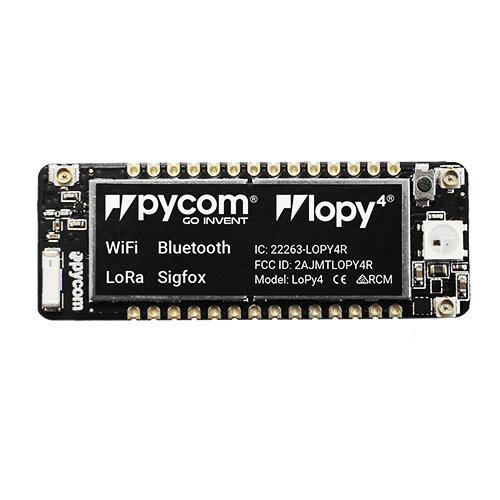
\includegraphics[keepaspectratio=true,scale=1.7]{pycom_lopy4.jpeg}
        \caption{pycom lopy 4}
  \end{minipage}
  \hfill
  \begin{minipage}[b]{0.4\textwidth}
   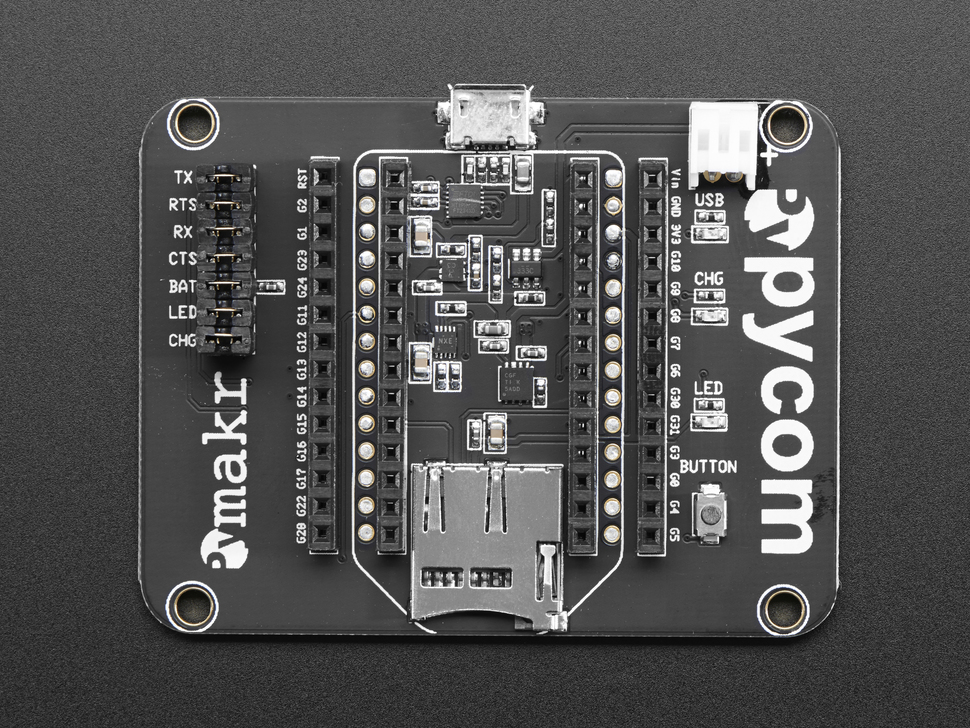
\includegraphics[keepaspectratio=true,scale=0.5]{pycom_expansion_board.jpeg}
    \caption{expansion board v3.0}
  \end{minipage}
\end{figure}

    \begin{figure}[H]
\begin{center}
\advance\leftskip-3cm
\advance\rightskip-3cm
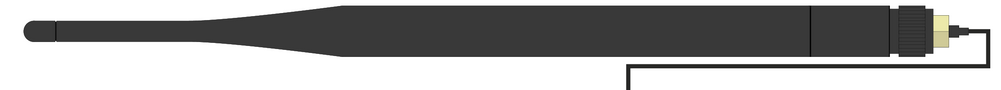
\includegraphics[keepaspectratio=true,scale=0.2]{lora_antenna.png}
\caption{antenne LoRa}
\label{visina8}
\end{center}\end{figure}



\section{Matériel}
\textcolor{red}{Branchez l'antenne LoRa avant d'alimenter la carte sinon la carte grille}





\section{Code pour Over The Air Activation}

Informations complémentaires : \url{https://docs.pycom.io/tutorials/lora/lorawan-nano-gateway/}\\

\textbf{Le code se trouve à : \url{https://github.com/GitClementtest/node_otaa}}

\subsection{Over The Air Activation}
Téléchargez le code suivant sur une carte lopy4+pymakr+antenne :

\begin{minted}{python}

""" OTAA Node example compatible with the LoPy Nano Gateway """

from network import LoRa
import socket
import ubinascii
import struct
import time

# Initialize LoRa in LORAWAN mode.
lora = LoRa(mode=LoRa.LORAWAN, region=LoRa.EU868)

# create an OTA authentication params
dev_eui = ubinascii.unhexlify('1111111111111111') # these settings can be found from TTN
app_eui = ubinascii.unhexlify('70B3D57ED00210CD') # these settings can be found from TTN
app_key = ubinascii.unhexlify('6C5401A22F121D96BBF13CF4B1871795') # these settings can 
#be found from TTN

# set the 3 default channels to the same frequency (must be before sending the OTAA 
#join request)
lora.add_channel(0, frequency=868100000, dr_min=0, dr_max=5)
lora.add_channel(1, frequency=868100000, dr_min=0, dr_max=5)
lora.add_channel(2, frequency=868100000, dr_min=0, dr_max=5)

# join a network using OTAA
lora.join(activation=LoRa.OTAA, auth=(dev_eui, app_eui, app_key), timeout=0)

# wait until the module has joined the network
while not lora.has_joined():
    time.sleep(2.5)
    print('Not joined yet...')

# remove all the non-default channels
for i in range(3, 16):
    lora.remove_channel(i)

# create a LoRa socket
s = socket.socket(socket.AF_LORA, socket.SOCK_RAW)

# set the LoRaWAN data rate
s.setsockopt(socket.SOL_LORA, socket.SO_DR, 5)

# make the socket non-blocking
s.setblocking(False)

time.sleep(5.0)

""" Your own code can be written below! """

for i in range (200):
    s.send(b'PKT #' + bytes([i]))
    time.sleep(4)
    rx = s.recv(256)
    if rx:
        print(rx)
    time.sleep(6)


\end{minted}

\subsection{Créer une application sur The Thing Network}

\begin{itemize}


    \item Créez une application
    Depuis \textit{Console} sélectionner application, puis ajoutez une application :
    
    
    \begin{figure}[H]
\begin{center}
\advance\leftskip-3cm
\advance\rightskip-3cm
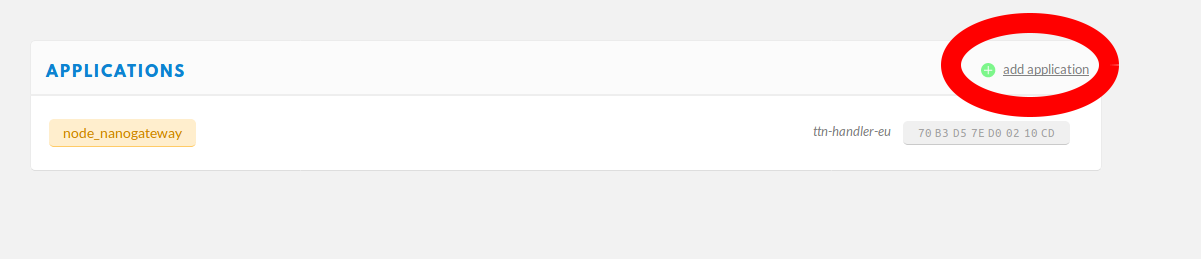
\includegraphics[keepaspectratio=true,scale=0.4]{add_appli.png}
\label{visina8}
\end{center}\end{figure}
    
    Donnez un nom pour l'application ID :
    
     \begin{figure}[H]
\begin{center}
\advance\leftskip-3cm
\advance\rightskip-3cm
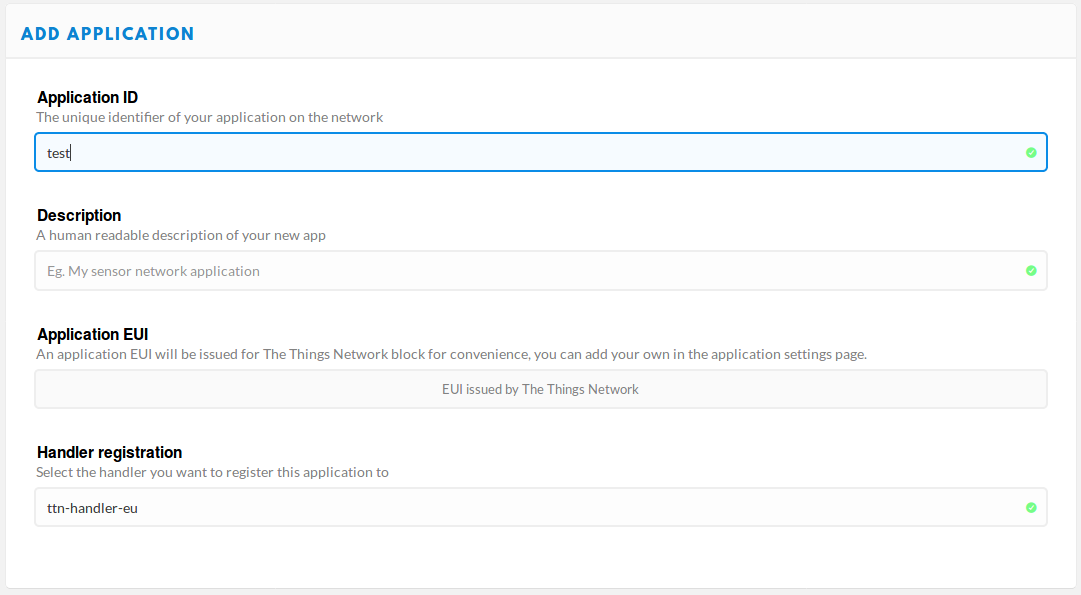
\includegraphics[keepaspectratio=true,scale=0.4]{appli_id.png}
\label{visina8}
\end{center}\end{figure}

\end{itemize}
    
    \subsection{Ajouter un device dans l'application}
    
        \begin{figure}[H]
\begin{center}
\advance\leftskip-3cm
\advance\rightskip-3cm
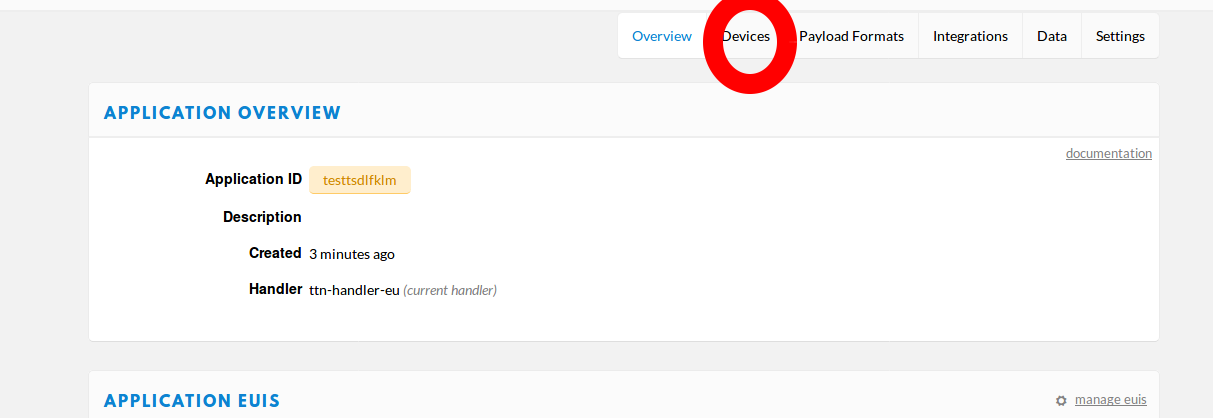
\includegraphics[keepaspectratio=true,scale=0.4]{add_device.png}
\label{visina8}
\end{center}\end{figure}

Puis \textit{register device} \\
Choisir un nom pour le device ID et 16 caractères hexadecimaux pour l'EUI.



 \begin{figure}[H]
\begin{center}
\advance\leftskip-3cm
\advance\rightskip-3cm
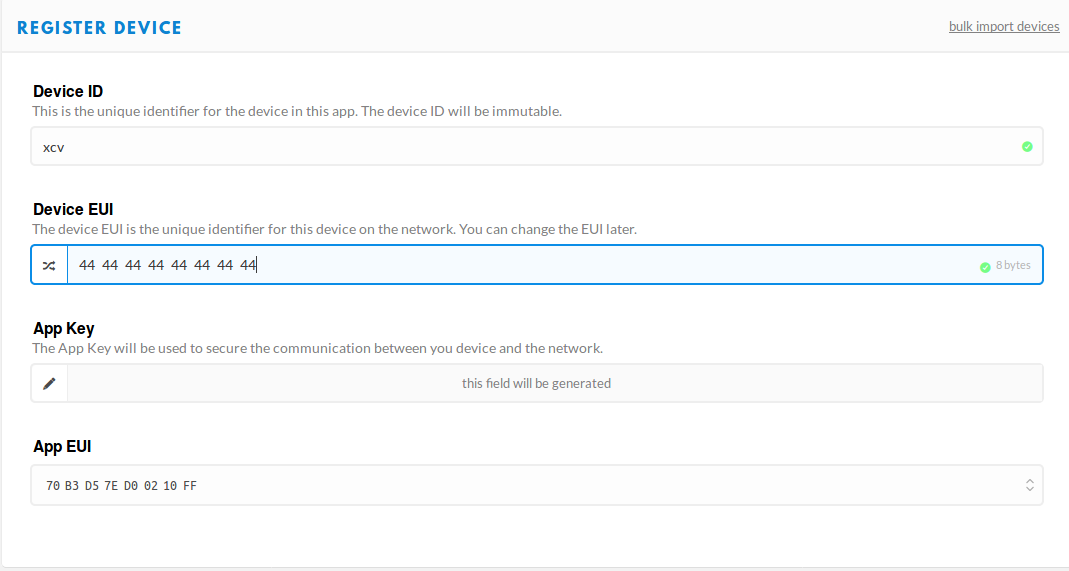
\includegraphics[keepaspectratio=true,scale=0.4]{device_eg.png}

\label{visina8}
\end{center}\end{figure}
 \textbf{Copiez les valeurs de Device EUI, APP Key et App EUI dans main.py}\\

 
 
 Choisir OTAA comme méthode d'activation
 
 
  \begin{figure}[H]
\begin{center}
\advance\leftskip-3cm
\advance\rightskip-3cm
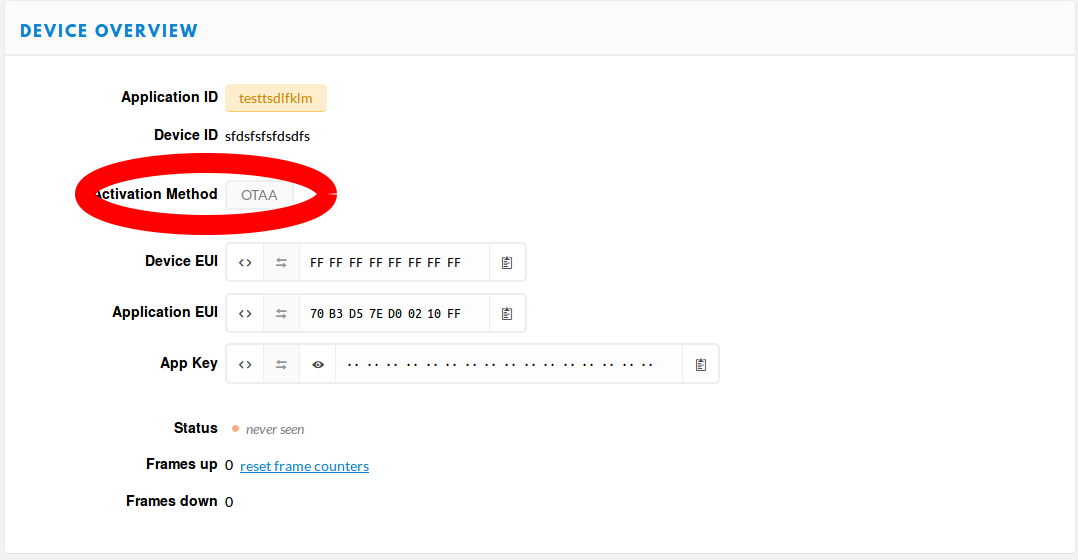
\includegraphics[keepaspectratio=true,scale=0.4]{device_overview.png}

\label{visina8}
\end{center}\end{figure}
 
 
Téléchargez le code sur la carte avec Atom. 
    
    
    \subsection{Lire la payload envoyée par le device}
    
    \begin{itemize}
    \item Une fois le device connecté :
    \begin{figure}[H]
\begin{center}
\advance\leftskip-3cm
\advance\rightskip-3cm
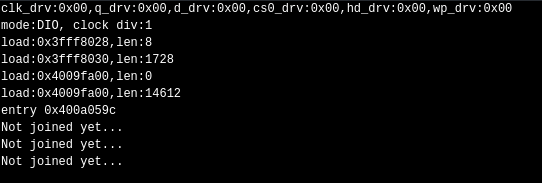
\includegraphics[keepaspectratio=true,scale=0.6]{nanogateway_node.png}
\caption{Atom}
\label{visina8}
\end{center}\end{figure}
 
  \begin{figure}[H]
\begin{center}
\advance\leftskip-3cm
\advance\rightskip-3cm
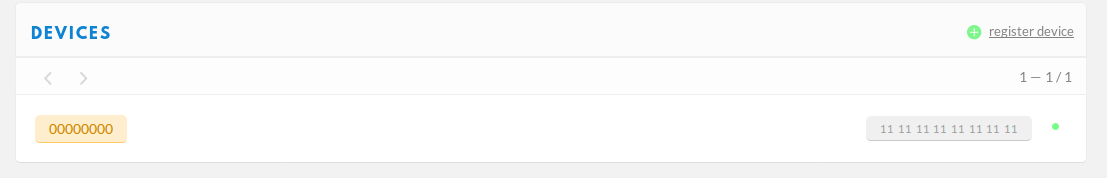
\includegraphics[keepaspectratio=true,scale=0.4]{device_connected.png}
\label{visina8}
\end{center}\end{figure}
  
  
  \item Dans l'onglet data :
  
  \begin{figure}[H]
\begin{center}
\advance\leftskip-3cm
\advance\rightskip-3cm
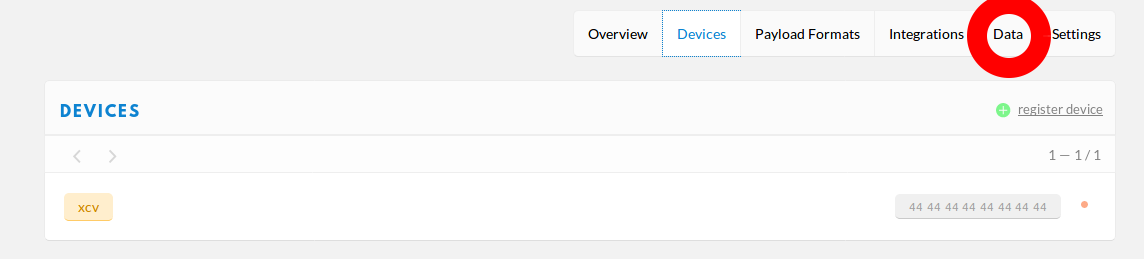
\includegraphics[keepaspectratio=true,scale=0.4]{data_tab.png}
\label{visina8}
\end{center}\end{figure}
  
  
  
  \begin{figure}[H]
\begin{center}
\advance\leftskip-3cm
\advance\rightskip-3cm
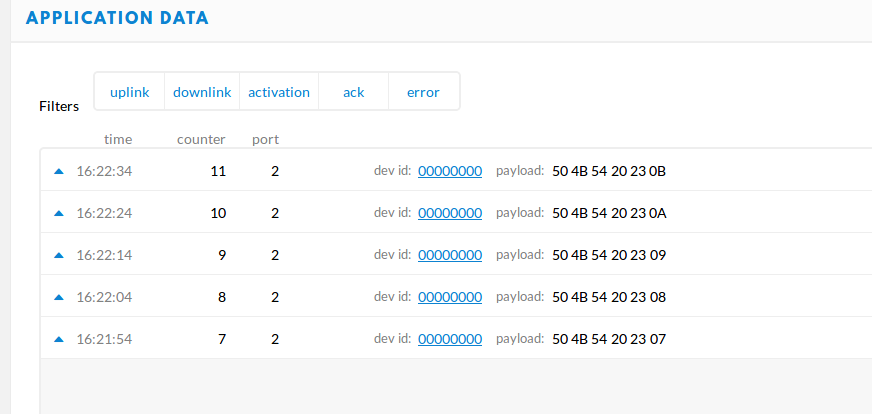
\includegraphics[keepaspectratio=true,scale=0.4]{payload.png}
\label{visina8}
\end{center}\end{figure}
  
  
\end{itemize}





\end{document}
